\documentclass{standalone}
\usepackage{tikz}
\usetikzlibrary{patterns, positioning}


\begin{document}
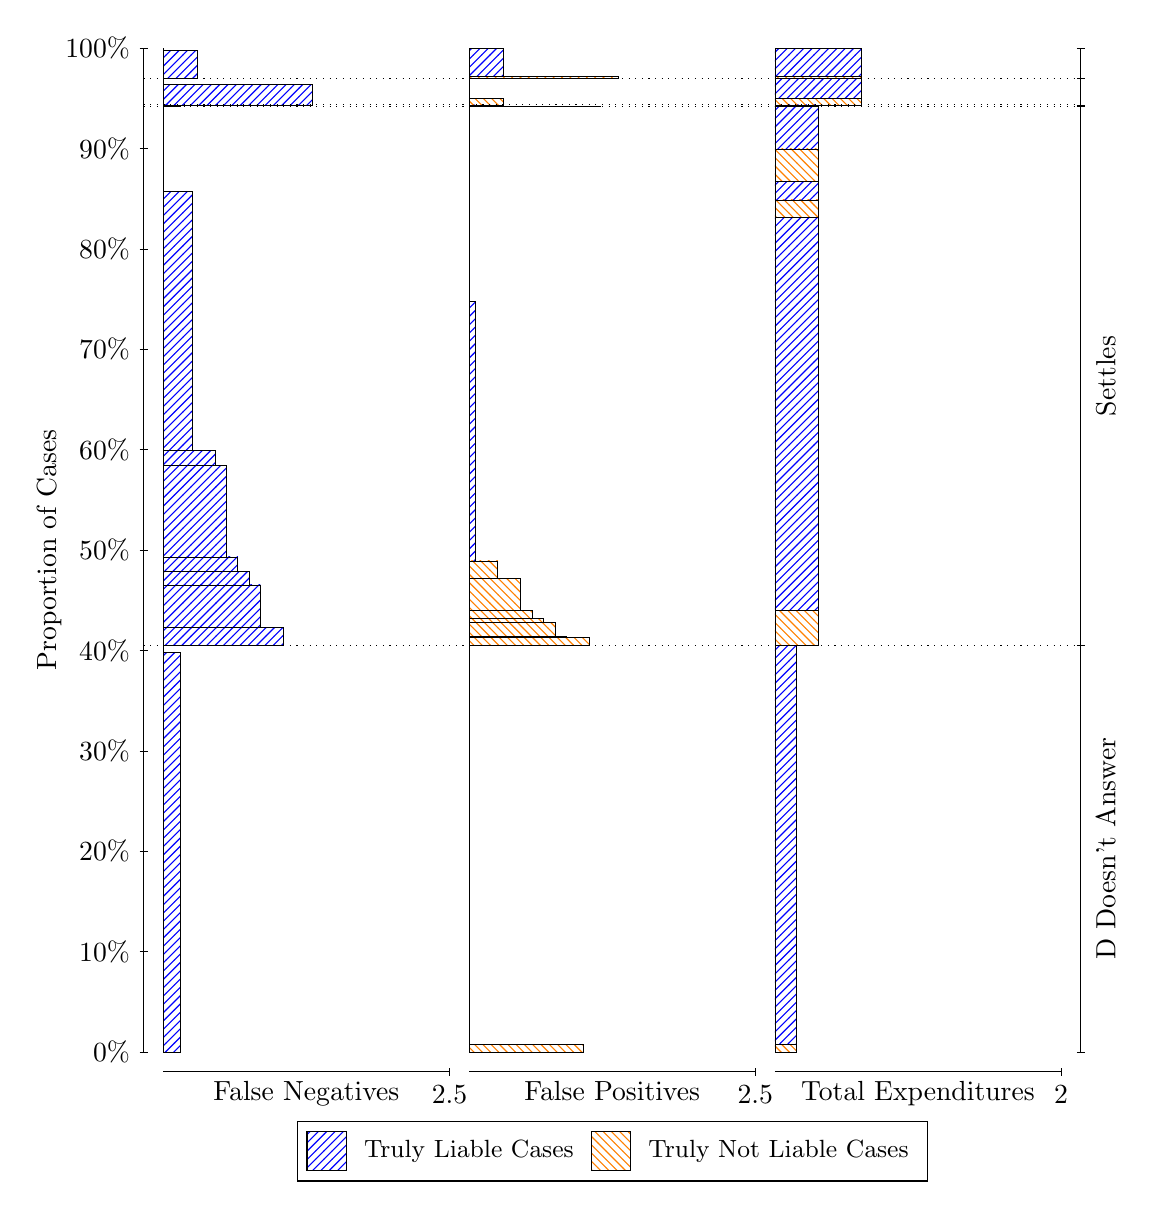
\begin{tikzpicture}
\draw[black, very thin] (1.5,1.75) -- (1.5,14.5);
\node[rotate=90, text=black, anchor=center] at (0.3, 8.125) {Proportion of Cases};
\draw[black, very thin] (1.45,1.75) -- (1.55,1.75);
\node[text=black, anchor=east] at (1.45, 1.75) {0\%};
\draw[black, very thin] (1.45,3.025) -- (1.55,3.025);
\node[text=black, anchor=east] at (1.45, 3.025) {10\%};
\draw[black, very thin] (1.45,4.3) -- (1.55,4.3);
\node[text=black, anchor=east] at (1.45, 4.3) {20\%};
\draw[black, very thin] (1.45,5.575) -- (1.55,5.575);
\node[text=black, anchor=east] at (1.45, 5.575) {30\%};
\draw[black, very thin] (1.45,6.85) -- (1.55,6.85);
\node[text=black, anchor=east] at (1.45, 6.85) {40\%};
\draw[black, very thin] (1.45,8.125) -- (1.55,8.125);
\node[text=black, anchor=east] at (1.45, 8.125) {50\%};
\draw[black, very thin] (1.45,9.4) -- (1.55,9.4);
\node[text=black, anchor=east] at (1.45, 9.4) {60\%};
\draw[black, very thin] (1.45,10.675) -- (1.55,10.675);
\node[text=black, anchor=east] at (1.45, 10.675) {70\%};
\draw[black, very thin] (1.45,11.95) -- (1.55,11.95);
\node[text=black, anchor=east] at (1.45, 11.95) {80\%};
\draw[black, very thin] (1.45,13.225) -- (1.55,13.225);
\node[text=black, anchor=east] at (1.45, 13.225) {90\%};
\draw[black, very thin] (1.45,14.5) -- (1.55,14.5);
\node[text=black, anchor=east] at (1.45, 14.5) {100\%};

\draw[black, very thin] (13.4,1.75) -- (13.4,14.5);
\draw[black, very thin] (13.35,1.75) -- (13.45,1.75);
\node[anchor=west] at (13.35, 1.75) {};
\draw[black, very thin] (13.35,6.9124) -- (13.45,6.9124);
\node[anchor=west] at (13.35, 6.9124) {};
\draw[black, very thin] (13.35,13.757) -- (13.45,13.757);
\node[anchor=west] at (13.35, 13.757) {};
\draw[black, very thin] (13.35,13.778) -- (13.45,13.778);
\node[anchor=west] at (13.35, 13.778) {};
\draw[black, very thin] (13.35,14.114) -- (13.45,14.114);
\node[anchor=west] at (13.35, 14.114) {};
\draw[black, very thin] (13.35,14.5) -- (13.45,14.5);
\node[anchor=west] at (13.35, 14.5) {};

\draw[black, very thin, pattern color=blue, pattern=north east lines] (1.75,1.75) rectangle (1.968,6.8208);
\draw[black, very thin, pattern color=orange, pattern=north west lines] (1.75,6.8208) rectangle (1.75,6.9124);
\draw[black, very thin, pattern color=blue, pattern=north east lines] (1.75,6.9124) rectangle (3.276,7.1456);
\draw[black, very thin, pattern color=blue, pattern=north east lines] (1.75,7.1456) rectangle (2.9853,7.6826);
\draw[black, very thin, pattern color=blue, pattern=north east lines] (1.75,7.6826) rectangle (2.84,7.8529);
\draw[black, very thin, pattern color=blue, pattern=north east lines] (1.75,7.8529) rectangle (2.6947,8.0374);
\draw[black, very thin, pattern color=blue, pattern=north east lines] (1.75,8.0374) rectangle (2.5493,9.2018);
\draw[black, very thin, pattern color=blue, pattern=north east lines] (1.75,9.2018) rectangle (2.404,9.3853);
\draw[black, very thin, pattern color=blue, pattern=north east lines] (1.75,9.3853) rectangle (2.1133,12.682);
\draw[black, very thin, pattern color=orange, pattern=north west lines] (1.75,12.682) rectangle (1.75,13.757);
\draw[black, very thin, pattern color=blue, pattern=north east lines] (1.75,13.757) rectangle (1.968,13.778);
\draw[black, very thin, pattern color=orange, pattern=north west lines] (1.75,13.778) rectangle (1.75,13.778);
\draw[black, very thin, pattern color=blue, pattern=north east lines] (1.75,13.778) rectangle (3.6393,14.034);
\draw[black, very thin, pattern color=orange, pattern=north west lines] (1.75,14.034) rectangle (1.75,14.114);
\draw[black, very thin, pattern color=blue, pattern=north east lines] (1.75,14.114) rectangle (2.186,14.472);
\draw[black, very thin, pattern color=orange, pattern=north west lines] (1.75,14.472) rectangle (1.75,14.5);
\draw[black, very thin, pattern color=orange, pattern=north west lines] (5.6333,1.75) rectangle (7.0867,1.8416);
\draw[black, very thin, pattern color=blue, pattern=north east lines] (5.6333,1.8416) rectangle (5.6333,6.9124);
\draw[black, very thin, pattern color=orange, pattern=north west lines] (5.6333,6.9124) rectangle (7.1593,7.0184);
\draw[black, very thin, pattern color=orange, pattern=north west lines] (5.6333,7.0184) rectangle (6.8687,7.0327);
\draw[black, very thin, pattern color=orange, pattern=north west lines] (5.6333,7.0327) rectangle (6.7233,7.2036);
\draw[black, very thin, pattern color=orange, pattern=north west lines] (5.6333,7.2036) rectangle (6.578,7.2595);
\draw[black, very thin, pattern color=orange, pattern=north west lines] (5.6333,7.2595) rectangle (6.4327,7.3546);
\draw[black, very thin, pattern color=orange, pattern=north west lines] (5.6333,7.3546) rectangle (6.2873,7.769);
\draw[black, very thin, pattern color=orange, pattern=north west lines] (5.6333,7.769) rectangle (5.9967,7.9866);
\draw[black, very thin, pattern color=blue, pattern=north east lines] (5.6333,7.9866) rectangle (5.706,11.284);
\draw[black, very thin, pattern color=blue, pattern=north east lines] (5.6333,11.284) rectangle (5.6333,13.757);
\draw[black, very thin, pattern color=orange, pattern=north west lines] (5.6333,13.757) rectangle (7.3047,13.757);
\draw[black, very thin, pattern color=blue, pattern=north east lines] (5.6333,13.757) rectangle (5.8513,13.778);
\draw[black, very thin, pattern color=orange, pattern=north west lines] (5.6333,13.778) rectangle (6.0693,13.859);
\draw[black, very thin, pattern color=blue, pattern=north east lines] (5.6333,13.859) rectangle (5.6333,14.114);
\draw[black, very thin, pattern color=orange, pattern=north west lines] (5.6333,14.114) rectangle (7.5227,14.142);
\draw[black, very thin, pattern color=blue, pattern=north east lines] (5.6333,14.142) rectangle (6.0693,14.5);
\draw[black, very thin, pattern color=orange, pattern=north west lines] (9.5167,1.75) rectangle (9.7892,1.8416);
\draw[black, very thin, pattern color=blue, pattern=north east lines] (9.5167,1.8416) rectangle (9.7892,6.9124);
\draw[black, very thin, pattern color=orange, pattern=north west lines] (9.5167,6.9124) rectangle (10.062,7.3546);
\draw[black, very thin, pattern color=blue, pattern=north east lines] (9.5167,7.3546) rectangle (10.062,12.354);
\draw[black, very thin, pattern color=orange, pattern=north west lines] (9.5167,12.354) rectangle (10.062,12.572);
\draw[black, very thin, pattern color=blue, pattern=north east lines] (9.5167,12.572) rectangle (10.062,12.805);
\draw[black, very thin, pattern color=orange, pattern=north west lines] (9.5167,12.805) rectangle (10.062,13.22);
\draw[black, very thin, pattern color=blue, pattern=north east lines] (9.5167,13.22) rectangle (10.062,13.757);
\draw[black, very thin, pattern color=orange, pattern=north west lines] (9.5167,13.757) rectangle (10.062,13.757);
\draw[black, very thin, pattern color=blue, pattern=north east lines] (9.5167,13.757) rectangle (10.062,13.778);
\draw[black, very thin, pattern color=orange, pattern=north west lines] (9.5167,13.778) rectangle (10.607,13.859);
\draw[black, very thin, pattern color=blue, pattern=north east lines] (9.5167,13.859) rectangle (10.607,14.114);
\draw[black, very thin, pattern color=orange, pattern=north west lines] (9.5167,14.114) rectangle (10.607,14.142);
\draw[black, very thin, pattern color=blue, pattern=north east lines] (9.5167,14.142) rectangle (10.607,14.5);
\draw[black, dotted] (1.5,6.9124) -- (13.4,6.9124);
\draw[black, dotted] (1.5,13.757) -- (13.4,13.757);
\draw[black, dotted] (1.5,13.778) -- (13.4,13.778);
\draw[black, dotted] (1.5,14.114) -- (13.4,14.114);
\draw[black, very thin] (1.75,1.5) -- (5.3833,1.5);
\node[text=black, anchor=north] at (3.5667, 1.5) {False Negatives};
\draw[black, very thin] (5.3833,1.45) -- (5.3833,1.55);
\node[text=black, anchor=north] at (5.3833, 1.45) {2.5};

\draw[black, very thin] (5.6333,1.5) -- (9.2667,1.5);
\node[text=black, anchor=north] at (7.45, 1.5) {False Positives};
\draw[black, very thin] (9.2667,1.45) -- (9.2667,1.55);
\node[text=black, anchor=north] at (9.2667, 1.45) {2.5};

\draw[black, very thin] (9.5167,1.5) -- (13.15,1.5);
\node[text=black, anchor=north] at (11.333, 1.5) {Total Expenditures};
\draw[black, very thin] (13.15,1.45) -- (13.15,1.55);
\node[text=black, anchor=north] at (13.15, 1.45) {2};

\node[text=black, centered, rotate=90] at (13.72, 4.3312) {D Doesn't Answer};
\node[text=black, centered, rotate=90] at (13.72, 10.334) {Settles};




\draw (7.449999999999999,1.5) node[draw=none] (baseCoordinate) {};
\begin{scope}[align=center]
        \matrix[scale=0.5, draw=black, below=0.5cm of baseCoordinate, nodes={draw}, column sep=0.1cm]{
            \node[rectangle, draw, minimum width=0.5cm, minimum height=0.5cm, pattern color=blue, pattern=north east lines] {}; &
            \node[draw=none, font=\small, text=black] (B) {Truly Liable Cases}; &
            \node[rectangle, draw, minimum width=0.5cm, minimum height=0.5cm, pattern color=orange, pattern=north west lines] {}; &
            \node[draw=none, font=\small, text=black] (B) {Truly Not Liable Cases}; \\
            };
\end{scope}

\end{tikzpicture}
\end{document}